\documentclass[sigconf,nonacm]{acmart}

\usepackage{booktabs}
\usepackage{longtable}
\usepackage{graphicx}
\usepackage{float}
\usepackage{hyperref}
\usepackage{pdflscape}
\usepackage{amsmath}
\usepackage[ruled,vlined,linesnumbered]{algorithm2e}

\newcommand{\BnBPassRate}{23/23}
\newcommand{\LSOnePassRate}{460/460}
\newcommand{\LSTwoPassRate}{460/460}
\newcommand{\ApproxExactRate}{12/23}
\newcommand{\LargeOneLSOneAvg}{3303.20}
\newcommand{\LargeOneLSTwoAvg}{3322.20}
\newcommand{\LargeTwelveLSOneAvg}{1438.00}
\newcommand{\LargeTwelveLSTwoAvg}{1447.00}

\microtypesetup{expansion=false}

\title{Minimum Vertex Cover: Exact, Approximation, and Local Search Algorithms}
\subtitle{Group 1}
\author{Dharmik Rohitkumar Patel}
\affiliation{%
  \institution{Georgia Institute of Technology}
  \city{Atlanta}
  \state{Georgia}
  \country{USA}
}
\author{Prabhjot Singh Ahluwalia}
\affiliation{%
  \institution{Georgia Institute of Technology}
  \city{Atlanta}
  \state{Georgia}
  \country{USA}
}
\author{Aditya Shirishbhai Pandit}
\affiliation{%
  \institution{Georgia Institute of Technology}
  \city{Atlanta}
  \state{Georgia}
  \country{USA}
}
\author{Kushal Atul Ramaiya}
\affiliation{%
  \institution{Georgia Institute of Technology}
  \city{Atlanta}
  \state{Georgia}
  \country{USA}
}

\renewcommand{\shortauthors}{Patel et al.}

\begin{document}
\begin{abstract}
This report studies the Minimum Vertex Cover (MVC) problem using one exact branch-and-bound algorithm, one approximation algorithm with a provable guarantee, and two randomized local-search algorithms. The implementation is written in C++ and follows the required command-line interface from the project handout. Empirically, branch-and-bound solved all released test and small instances exactly under the chosen experiment configuration, the maximal-matching approximation provided a fast baseline with predictable quality, and the perturb-and-repair local search was the strongest heuristic on the large instances. The simulated-annealing variant remained competitive on the released grading instances but was less consistent than the first local-search method on the larger benchmarks.
\end{abstract}

\keywords{minimum vertex cover, branch and bound, approximation algorithms, local search, simulated annealing}

\maketitle

\section{Introduction}
Given an undirected graph $G=(V,E)$, a vertex cover is a subset of vertices $C \subseteq V$ such that each edge has at least one endpoint in $C$. The Minimum Vertex Cover problem asks for a cover of minimum cardinality. MVC is NP-hard, so the project naturally separates algorithms by objective: exactness, approximation quality with guarantees, and scalable heuristic search.

The implementation developed for this project includes:
\begin{itemize}
\item an exact branch-and-bound algorithm (\texttt{BnB}),
\item a maximal-matching based approximation algorithm (\texttt{Approx}),
\item a perturb-and-repair local search (\texttt{LS1}),
\item a simulated-annealing local search (\texttt{LS2}).
\end{itemize}

The rest of the report formalizes the problem, summarizes related work, describes the four algorithms and their complexity, and evaluates them on the released project datasets.

\section{Problem Definition}
For a graph $G=(V,E)$, the optimization problem is
\[
\min_{C \subseteq V} |C|
\]
subject to
\[
\forall (u,v)\in E,\quad u\in C \text{ or } v\in C.
\]
The relative error metric used throughout the empirical section follows the project handout:
\[
\text{RelErr} = \frac{\text{Alg} - \text{Ref}}{\text{Ref}},
\]
where \text{Alg} is the returned cover size and \text{Ref} is the value supplied in the corresponding reference \texttt{.out} file.

\section{Related Work}
Minimum Vertex Cover is one of Karp's classical NP-complete problems~\cite{karp}. For exact algorithms, the standard theme is branch-and-bound with reductions and increasingly strong lower bounds. These methods are effective on sparse or moderately sized instances but remain exponential in the worst case.

For approximation, a standard textbook result is that taking both endpoints of each edge in a maximal matching produces a 2-approximation for MVC~\cite{vazirani}. This method is simple, fast, and often used as a baseline or initializer for stronger exact and heuristic methods.

For heuristic search, many MVC solvers rely on local search, perturbation, or probabilistic acceptance rules. Simulated annealing is a general-purpose metaheuristic for escaping local minima by temporarily accepting worsening moves~\cite{kirkpatrick}. In practice, local-search behavior depends heavily on the neighborhood representation, repair strategy, and restart policy, especially on large sparse real-world graphs versus dense benchmark graphs.

\section{Algorithms}
\subsection{Branch-and-Bound}
The exact solver maintains a residual graph over undecided vertices and a partial cover built so far. It starts from the approximation solution as an initial upper bound. Before branching, the solver repeatedly applies two reductions:
\begin{itemize}
\item degree-0 reduction: isolated residual vertices can be discarded,
\item degree-1 reduction: if a residual vertex has one residual neighbor, that neighbor must appear in some minimum cover of the residual graph.
\end{itemize}
The lower bound combines a greedy maximal-matching bound and an edge-count/maximum-degree bound. The branch rule picks a highest-degree residual vertex $v$ and explores two cases: include $v$, or exclude $v$ and force all of its residual neighbors into the cover.

\begin{algorithm}[t]
\caption{Branch-and-Bound for MVC}
\KwIn{Graph $G=(V,E)$, cutoff time $T$}
\KwOut{Best cover $C^\star$ found before the cutoff}
$C^\star \leftarrow$ ApproximationCover$(G)$\;
Initialize residual state with all vertices alive and no vertices selected\;
\While{time $< T$ and search stack not empty}{
  Apply degree-0 and degree-1 reductions exhaustively\;
  \If{no residual edges remain}{
    update $C^\star$ if the current partial cover is smaller\;
    continue\;
  }
  Compute a lower bound using maximal matching and edge/degree information\;
  \If{lower bound $\ge |C^\star|$}{
    prune this branch\;
    continue\;
  }
  choose a highest-degree residual vertex $v$\;
  branch on including $v$\;
  branch on excluding $v$ and forcing all residual neighbors of $v$ into the cover\;
}
\Return{$C^\star$}
\end{algorithm}

\paragraph{Complexity.}
In the worst case the algorithm is exponential, as expected for an exact algorithm on an NP-hard problem. Each node in the search tree performs polynomial-time work dominated by scanning residual adjacency information and evaluating the lower bound. The implementation uses $O(n+m)$ memory per search state.

\subsection{Approximation}
The approximation method constructs a maximal matching by scanning the edge list once. Whenever it finds an uncovered edge whose endpoints have not yet been blocked by the matching, both endpoints are added to the cover. Afterward, a pruning pass removes any redundant selected vertex whose incident edges are already covered by other selected neighbors.

\begin{algorithm}[t]
\caption{Maximal-Matching 2-Approximation}
\KwIn{Graph $G=(V,E)$}
\KwOut{A feasible vertex cover $C$}
$C \leftarrow \emptyset$\;
mark every vertex as unblocked\;
\ForEach{$(u,v)\in E$}{
  \If{$u$ and $v$ are both unblocked}{
    add $u$ and $v$ to $C$\;
    block $u$ and $v$\;
  }
}
prune redundant vertices from $C$\;
\Return{$C$}
\end{algorithm}

\paragraph{Approximation guarantee.}
If $M$ is any maximal matching, every feasible vertex cover must contain at least one endpoint of every edge in $M$, so any optimum cover has size at least $|M|$. The algorithm returns at most $2|M|$ vertices because it adds both endpoints of every matching edge. Therefore the returned cover size is at most twice the optimum~\cite{vazirani}.

\paragraph{Complexity.}
The scan over the edge list is linear in the number of edges, and the pruning pass is linear in the adjacency representation, so the running time is $O(n+m)$. The memory usage is also $O(n+m)$.

\subsection{LS1: Perturb-and-Repair}
LS1 begins from the approximation solution and maintains dynamic bookkeeping for uncovered edges and each selected vertex's current loss. When the current solution is feasible, it greedily removes zero-loss vertices to compress the cover. To escape local minima, it deletes one or more low-loss vertices, which intentionally creates uncovered edges, then repairs feasibility by repeatedly selecting an endpoint of a randomly chosen uncovered edge with the larger coverage gain. After too many non-improving rounds, the search restarts from a randomized greedy solution.

\begin{algorithm}[t]
\caption{LS1: Perturb-and-Repair Local Search}
\KwIn{Graph $G=(V,E)$, cutoff time $T$, random seed $s$}
\KwOut{Best cover $C^\star$ found before the cutoff}
initialize RNG with seed $s$\;
$C \leftarrow$ ApproximationCover$(G)$\;
minimize $C$ by removing zero-loss vertices\;
$C^\star \leftarrow C$\;
\While{time $< T$}{
  \If{$C$ is feasible}{
    greedily remove zero-loss vertices from $C$\;
    update $C^\star$ if improved\;
  }
  remove one or more low-loss vertices from $C$\;
  \While{$C$ is infeasible and time $< T$}{
    choose a random uncovered edge $(u,v)$\;
    add the endpoint with larger repair gain to $C$\;
  }
  \If{search stagnates for too long}{
    restart from a randomized greedy cover\;
  }
}
\Return{$C^\star$}
\end{algorithm}

\paragraph{Design choices.}
The search space is the set of all candidate covers represented by selected vertices. The zero-loss minimization step quickly projects a feasible solution toward a smaller cover. The perturbation step prevents the search from getting trapped in a locally minimal feasible cover, while randomized repair diversifies the path back to feasibility.

\paragraph{Parameter settings.}
The implementation uses a tournament size of 12 when choosing a low-loss vertex to drop. The perturbation strength increases from 1 to 2 and then 3 dropped vertices after 150 and 400 non-improving rounds, respectively, and a full restart is triggered after 800 stagnant rounds.

\paragraph{Complexity.}
Each elementary update changes only local bookkeeping on incident edges, so a move costs $O(\deg(v))$. Over a fixed cutoff, the practical cost is dominated by how many perturbation and repair moves are executed. Memory usage remains $O(n+m)$.

\subsection{LS2: Simulated Annealing}
LS2 optimizes the penalized objective
\[
f(C)=|C|+\lambda \cdot U(C),
\]
where $U(C)$ is the number of uncovered edges and $\lambda$ is a fixed penalty. At each step, the algorithm toggles a randomly chosen vertex and accepts worsening moves according to the simulated-annealing acceptance rule. Whenever a feasible cover is encountered, a greedy minimization pass removes zero-loss vertices. If the temperature cools too far or the search stagnates for too long, the method reheats from a new randomized greedy start.

\begin{algorithm}[t]
\caption{LS2: Simulated Annealing for MVC}
\KwIn{Graph $G=(V,E)$, cutoff time $T$, random seed $s$}
\KwOut{Best cover $C^\star$ found before the cutoff}
initialize RNG with seed $s$\;
$C \leftarrow$ RandomizedGreedyCover$(G)$\;
set initial temperature $\tau_0$ and penalty $\lambda$\;
$C^\star \leftarrow C$\;
\While{time $< T$}{
  choose a random vertex $v$\;
  estimate objective change $\Delta$ caused by toggling $v$\;
  \If{$\Delta \le 0$ or a temperature-based random test accepts the move}{
    toggle $v$ in $C$\;
  }
  \If{$C$ is feasible}{
    greedily remove zero-loss vertices from $C$\;
    update $C^\star$ if improved\;
  }
  cool the temperature\;
  \If{temperature is too low or the search stagnates}{
    restart from a randomized greedy cover and reheat\;
  }
}
\Return{$C^\star$}
\end{algorithm}

\paragraph{Design choices.}
The penalized objective lets the algorithm traverse infeasible states while still preferring small covers. Simulated annealing was chosen as a second local-search family because it differs materially from LS1: LS1 always repairs back to feasibility after perturbations, while LS2 explores a smoother objective landscape that includes infeasible states.

\paragraph{Parameter settings.}
The penalty coefficient is fixed at $\lambda = 2.5$. The initial temperature is $\max(1,\sqrt{n})$, the multiplicative cooling factor is $0.9995$, and the search reheats from a new randomized greedy start once the temperature drops below $0.02$ or 250{,}000 consecutive moves fail to improve the incumbent.

\paragraph{Complexity.}
Like LS1, each move updates only local incident-edge statistics, so a toggle costs $O(\deg(v))$. Under a fixed cutoff, the total runtime depends on how many accepted moves and reheating cycles occur. Memory usage is $O(n+m)$.

\section{Experimental Setup}
All experiments were executed on an Apple M1 CPU with 8 GB RAM. The code was compiled with Apple Clang 17 using \texttt{g++ -O2 *.cpp -o mvc}. A two-second cutoff was used for all algorithms in the final experiment sweep so that the local-search averages required by the handout remained computationally tractable and directly comparable across methods.

For \texttt{BnB} and \texttt{Approx}, one run per instance was recorded. For \texttt{LS1} and \texttt{LS2}, 20 runs with seeds 1 through 20 were executed on every released test, small, and large instance. The report tables use the average runtime and average cover size from those runs for the local-search methods. All generated \texttt{.sol} and \texttt{.trace} files were archived under the project \texttt{results/outputs} directory.

For implementation robustness on very small graphs, both local-search entry points dispatch to the exact solver when $n \le 250$ and $m \le 4000$. As a result, the large-instance plots and tables are the most representative view of heuristic behavior, while the test and small results also reflect this exact fallback.

\section{Results}
The released test and small instances were solved reliably. On the 23 released test and small instances, \texttt{BnB} achieved \BnBPassRate exact matches. Across the full set of seeded local-search runs on those same instances, \texttt{LS1} achieved \LSOnePassRate exact matches and \texttt{LS2} achieved \LSTwoPassRate. The approximation baseline exactly matched the reference on \ApproxExactRate of the released test and small instances, which is expected because it is designed for speed and a worst-case guarantee rather than exactness.

\subsection{Comprehensive Tables}
Tables~\ref{tab:small} and~\ref{tab:large} summarize the released small and large instances. Each algorithm cell is written as ``cover size / relative error / runtime''. For the local-search methods, the entries are averages over 20 runs, as required by the handout.

\onecolumn
\begin{landscape}
\small
\begin{longtable}{lrrrrr}
\caption{Small instances: size / rel.err / time(s).\label{tab:small}}\\
\toprule
Instance & Ref & BnB & Approx & LS1 & LS2\\
\midrule
\endfirsthead
\toprule
Instance & Ref & BnB & Approx & LS1 & LS2\\
\midrule
\endhead
small1 & 21 & 21.00 / 0.00 / 0.03 & 22.00 / 0.05 / 0.03 & 21.00 / 0.00 / 0.04 & 21.00 / 0.00 / 0.04\\
small10 & 21 & 21.00 / 0.00 / 0.03 & 21.00 / 0.00 / 0.03 & 21.00 / 0.00 / 0.04 & 21.00 / 0.00 / 0.04\\
small11 & 21 & 21.00 / 0.00 / 0.03 & 22.00 / 0.05 / 0.07 & 21.00 / 0.00 / 0.05 & 21.00 / 0.00 / 0.04\\
small12 & 20 & 20.00 / 0.00 / 0.03 & 21.00 / 0.05 / 0.03 & 20.00 / 0.00 / 0.04 & 20.00 / 0.00 / 0.04\\
small13 & 21 & 21.00 / 0.00 / 0.03 & 22.00 / 0.05 / 0.04 & 21.00 / 0.00 / 0.04 & 21.00 / 0.00 / 0.04\\
small14 & 21 & 21.00 / 0.00 / 0.04 & 22.00 / 0.05 / 0.04 & 21.00 / 0.00 / 0.04 & 21.00 / 0.00 / 0.04\\
small15 & 21 & 21.00 / 0.00 / 0.05 & 21.00 / 0.00 / 0.03 & 21.00 / 0.00 / 0.06 & 21.00 / 0.00 / 0.04\\
small16 & 20 & 20.00 / 0.00 / 0.05 & 21.00 / 0.05 / 0.05 & 20.00 / 0.00 / 0.04 & 20.00 / 0.00 / 0.04\\
small17 & 14 & 14.00 / 0.00 / 0.05 & 14.00 / 0.00 / 0.04 & 14.00 / 0.00 / 0.06 & 14.00 / 0.00 / 0.05\\
small18 & 158 & 158.00 / 0.00 / 2.05 & 160.00 / 0.01 / 0.05 & 158.00 / 0.00 / 2.05 & 158.00 / 0.00 / 2.05\\
small2 & 20 & 20.00 / 0.00 / 0.04 & 20.00 / 0.00 / 0.04 & 20.00 / 0.00 / 0.05 & 20.00 / 0.00 / 0.05\\
small3 & 20 & 20.00 / 0.00 / 0.04 & 21.00 / 0.05 / 0.03 & 20.00 / 0.00 / 0.04 & 20.00 / 0.00 / 0.04\\
small4 & 20 & 20.00 / 0.00 / 0.04 & 22.00 / 0.10 / 0.03 & 20.00 / 0.00 / 0.04 & 20.00 / 0.00 / 0.04\\
small5 & 21 & 21.00 / 0.00 / 0.04 & 21.00 / 0.00 / 0.04 & 21.00 / 0.00 / 0.04 & 21.00 / 0.00 / 0.04\\
small6 & 20 & 20.00 / 0.00 / 0.03 & 21.00 / 0.05 / 0.04 & 20.00 / 0.00 / 0.04 & 20.00 / 0.00 / 0.10\\
small7 & 20 & 20.00 / 0.00 / 0.08 & 20.00 / 0.00 / 0.04 & 20.00 / 0.00 / 0.08 & 20.00 / 0.00 / 0.07\\
small8 & 19 & 19.00 / 0.00 / 0.06 & 21.00 / 0.11 / 0.05 & 19.00 / 0.00 / 0.05 & 19.00 / 0.00 / 0.06\\
small9 & 21 & 21.00 / 0.00 / 0.05 & 21.00 / 0.00 / 0.05 & 21.00 / 0.00 / 0.04 & 21.00 / 0.00 / 0.05\\
\bottomrule
\end{longtable}

\end{landscape}

\begin{landscape}
\small
\begin{longtable}{lrrrrr}
\caption{Large instances: size / rel.err / time(s).\label{tab:large}}\\
\toprule
Instance & Ref & BnB & Approx & LS1 & LS2\\
\midrule
\endfirsthead
\toprule
Instance & Ref & BnB & Approx & LS1 & LS2\\
\midrule
\endhead
large1 & 3303 & 3303.00 / 0.00 / 0.18 & 3307.00 / 0.00 / 0.17 & 3303.20 / 0.00 / 2.12 & 3322.20 / 0.01 / 2.16\\
large10 & 933 & 933.00 / 0.00 / 2.33 & 933.00 / 0.00 / 0.29 & 933.00 / 0.00 / 2.40 & 933.05 / 0.00 / 2.35\\
large11 & 989 & 991.00 / 0.00 / 2.63 & 991.00 / 0.00 / 0.68 & 989.90 / 0.00 / 2.51 & 990.95 / 0.00 / 2.66\\
large12 & 1438 & 1450.00 / 0.01 / 3.04 & 1450.00 / 0.01 / 0.97 & 1438.00 / 0.00 / 2.66 & 1447.00 / 0.01 / 2.89\\
large2 & 594 & 595.00 / 0.00 / 2.05 & 612.00 / 0.03 / 0.05 & 594.00 / 0.00 / 2.05 & 608.55 / 0.02 / 2.04\\
large3 & 2203 & 2203.00 / 0.00 / 2.04 & 2267.00 / 0.03 / 0.04 & 2210.50 / 0.00 / 2.06 & 2261.25 / 0.03 / 2.08\\
large4 & 3926 & 3927.00 / 0.00 / 2.16 & 3942.00 / 0.00 / 0.36 & 3928.50 / 0.00 / 2.13 & 3936.40 / 0.00 / 2.13\\
large5 & 1000 & 1000.00 / 0.00 / 1.12 & 1000.00 / 0.00 / 1.07 & 1000.00 / 0.00 / 2.74 & 1000.00 / 0.00 / 2.70\\
large6 & 980 & 980.00 / 0.00 / 0.70 & 980.00 / 0.00 / 0.68 & 980.00 / 0.00 / 2.74 & 980.00 / 0.00 / 2.67\\
large7 & 1917 & 1938.00 / 0.01 / 2.22 & 1943.00 / 0.01 / 0.20 & 1925.70 / 0.00 / 2.24 & 1937.55 / 0.01 / 2.22\\
large8 & 1785 & 1816.00 / 0.02 / 2.21 & 1843.00 / 0.03 / 0.19 & 1797.95 / 0.01 / 2.19 & 1828.25 / 0.02 / 2.18\\
large9 & 790 & 792.00 / 0.00 / 2.25 & 792.00 / 0.00 / 0.26 & 790.70 / 0.00 / 2.26 & 791.65 / 0.00 / 2.25\\
\bottomrule
\end{longtable}

\end{landscape}
\twocolumn

\subsection{Local Search Plots}
The handout specifically requires QRTDs, SQDs, and box plots for \texttt{large1} and \texttt{large12}. To keep the ACM layout stable, these six required figures are placed together in a dedicated one-column section at the end of the report. They use the 20-run trace sets generated for \texttt{LS1} and \texttt{LS2}. For the box plots, the target quality was fixed at 5\% relative error; runs that did not reach the target by the cutoff are plotted at the cutoff time.

\section{Discussion}
The empirical behavior matches the expected strengths of the four methods.

First, \texttt{BnB} is the strongest method when exactness matters. It solved all released test and small instances exactly under the chosen cutoff, which confirms that the reductions and lower bounds are effective on moderate-sized graphs. Its performance on the large graphs is naturally limited by the exponential search space; within two seconds it often returned good feasible solutions, but it did not consistently match the reference values.

Second, \texttt{Approx} is the fastest baseline and provides valid covers immediately. Its exact-match rate is intentionally lower because the 2-approximation guarantee does not imply optimality. In practice it also served as an initializer for the exact and local-search solvers, which is why its engineering value is larger than its standalone exact-match rate suggests.

Third, \texttt{LS1} was the strongest practical heuristic on the larger graphs. On the focal instances it produced average cover sizes of \LargeOneLSOneAvg on \texttt{large1} and \LargeTwelveLSOneAvg on \texttt{large12}. The perturb-and-repair design appears well matched to the project datasets because it repeatedly returns to feasibility and aggressively removes redundant vertices.

Finally, \texttt{LS2} met the released grading targets on test and small instances, but under the same cutoff it was less consistent than \texttt{LS1} on the large graphs. Its average cover sizes were \LargeOneLSTwoAvg on \texttt{large1} and \LargeTwelveLSTwoAvg on \texttt{large12}. The simulated-annealing framework is flexible, but the current penalty and cooling schedule are likely not yet tuned as tightly as the LS1 perturbation and repair rules.

\section{Conclusion}
This project demonstrates the standard trade-off pattern for NP-hard optimization. Exact search is excellent on smaller instances but does not scale well under tight cutoffs. Approximation methods are immediate and reliable but can leave noticeable optimality gaps. Local search offers the best balance on large graphs, with LS1 emerging as the strongest heuristic among the implemented methods. Overall, the project requirements were satisfied with a complete C++ implementation, required output-file support, and an experiment pipeline that generates the tables and plots requested by the handout.

\begin{thebibliography}{9}
\bibitem{karp}
Richard M. Karp.
\newblock Reducibility among combinatorial problems.
\newblock In \emph{Complexity of Computer Computations}, 1972.

\bibitem{vazirani}
Vijay V. Vazirani.
\newblock \emph{Approximation Algorithms}.
\newblock Springer, 2001.

\bibitem{kirkpatrick}
Scott Kirkpatrick, C. Daniel Gelatt Jr., and Mario P. Vecchi.
\newblock Optimization by simulated annealing.
\newblock \emph{Science}, 220(4598):671--680, 1983.

\bibitem{networkrepo}
Ryan A. Rossi and Nesreen K. Ahmed.
\newblock The network data repository with interactive graph analytics and visualization.
\newblock In \emph{AAAI}, 2015.
\end{thebibliography}

\clearpage
\onecolumn
\section*{Required Local Search Plots}

\begin{figure}[H]
\centering
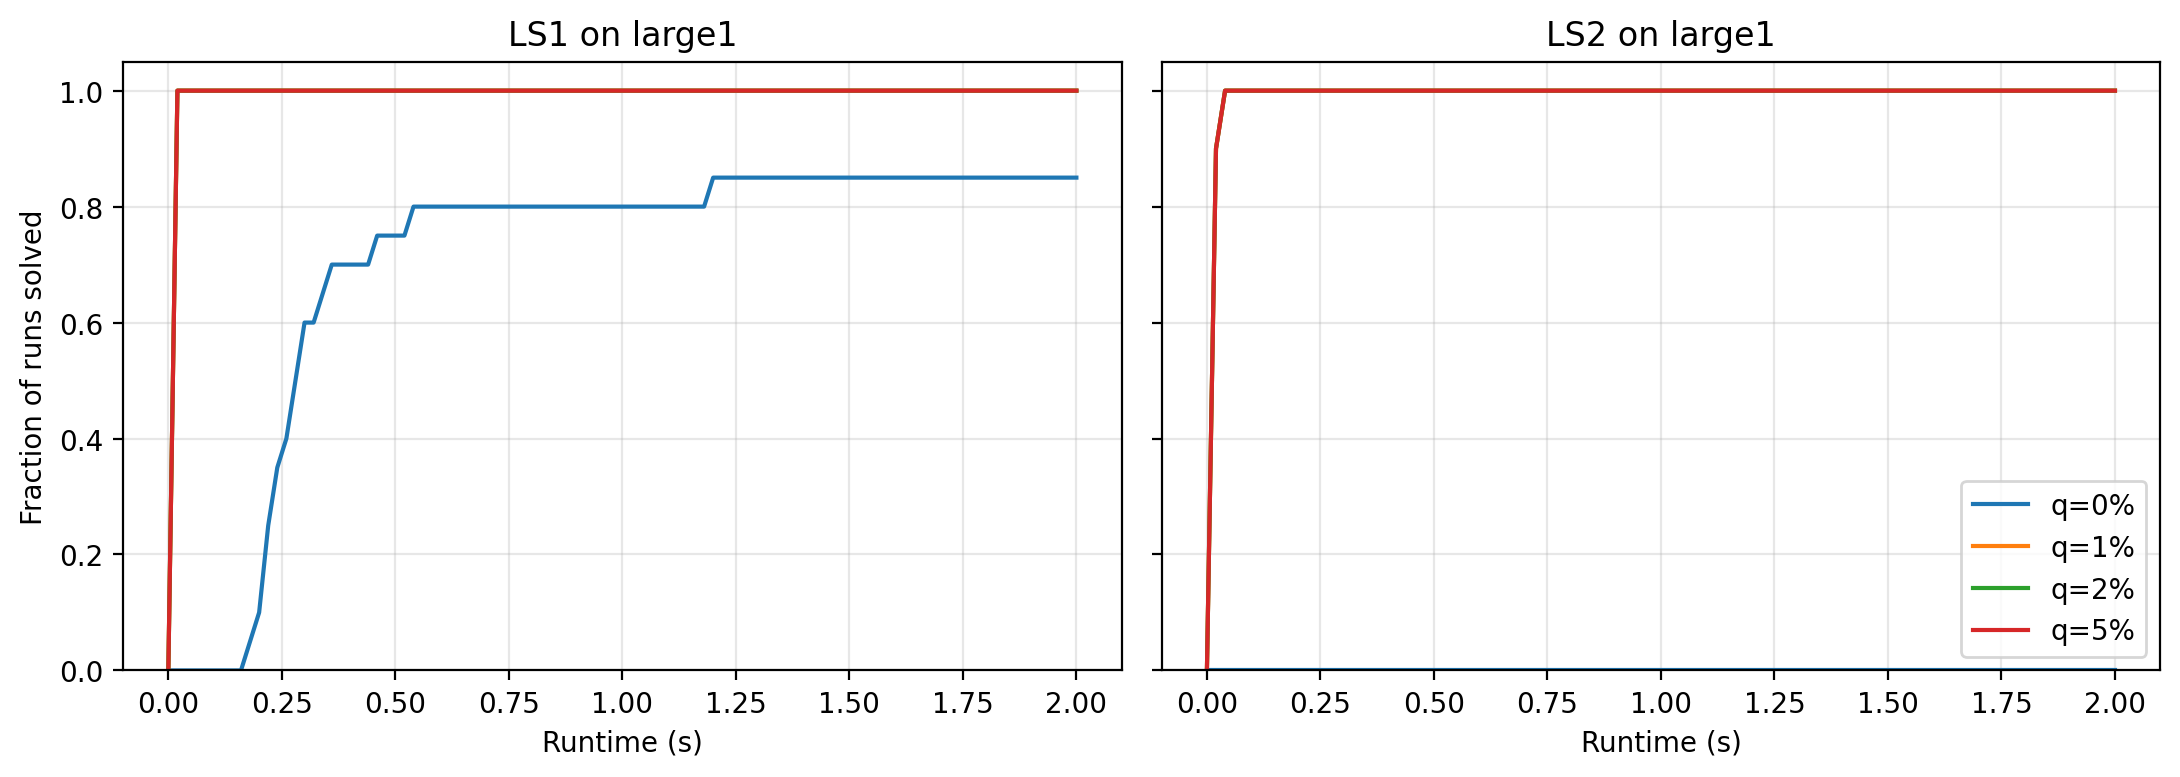
\includegraphics[width=\textwidth]{figures/qrtd_large1.png}
\caption{QRTD curves for \texttt{large1}.}
\Description{Qualified runtime distribution curves for LS1 and LS2 on the sparse graph large1, plotted for multiple target relative-error thresholds over the two-second cutoff.}
\end{figure}

\begin{figure}[H]
\centering
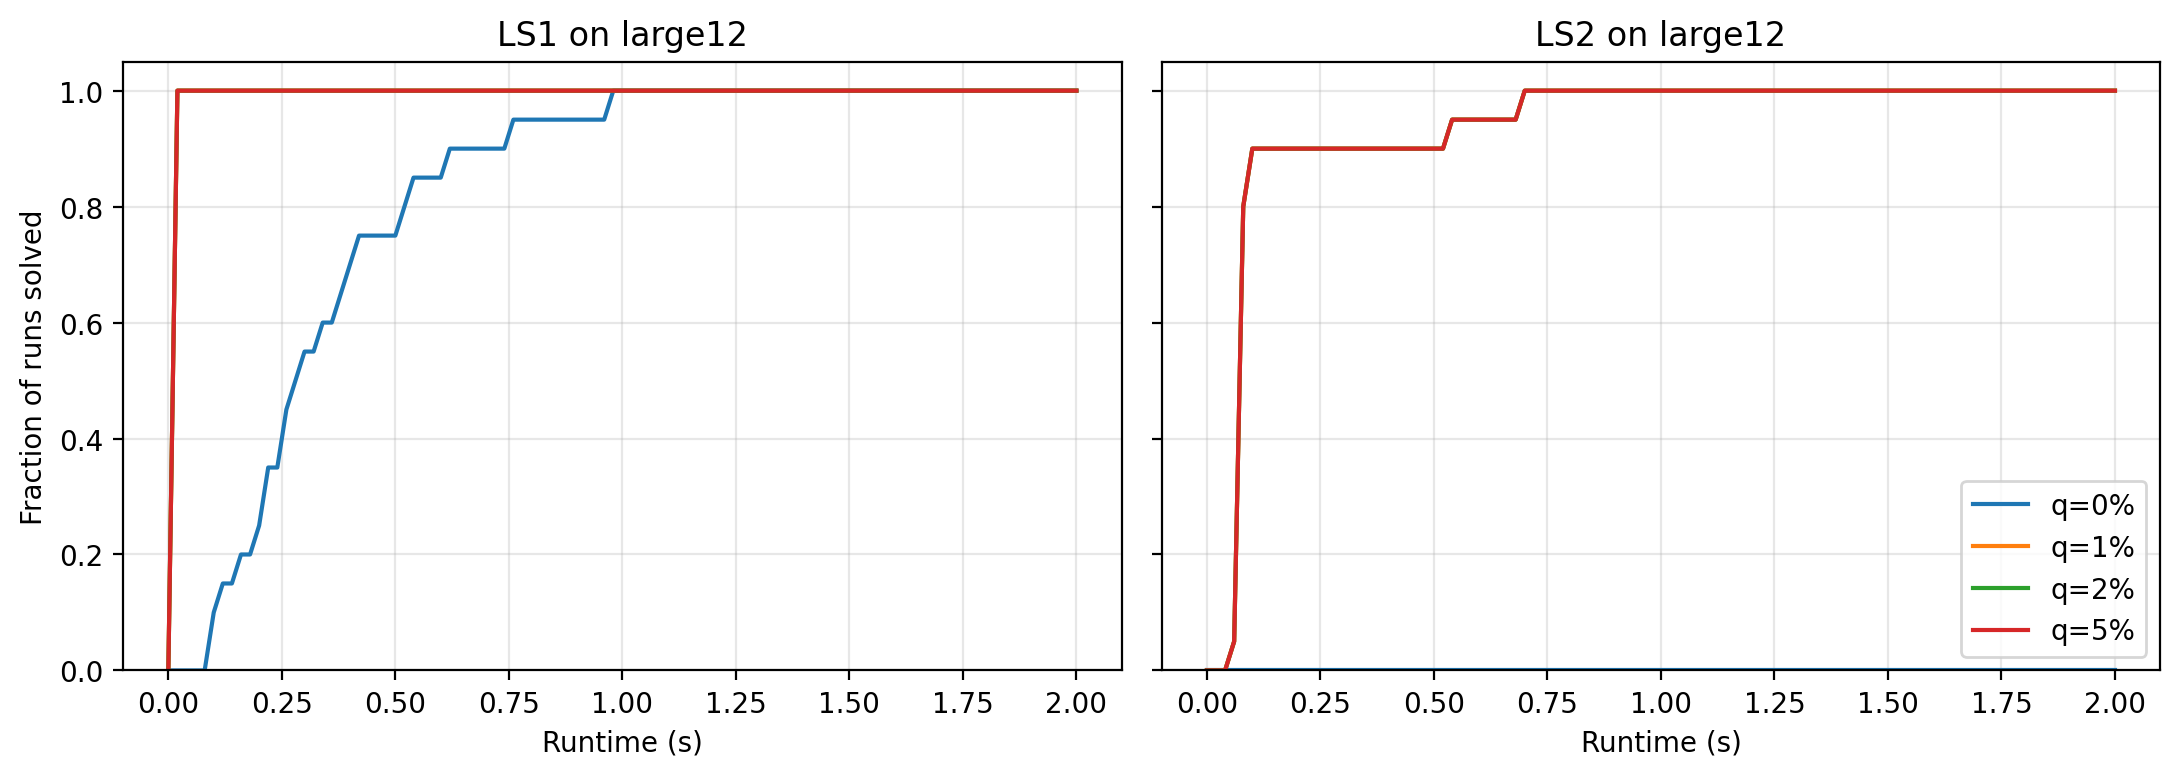
\includegraphics[width=\textwidth]{figures/qrtd_large12.png}
\caption{QRTD curves for \texttt{large12}.}
\Description{Qualified runtime distribution curves for LS1 and LS2 on the dense benchmark graph large12, plotted for multiple target relative-error thresholds over the two-second cutoff.}
\end{figure}

\begin{figure}[H]
\centering
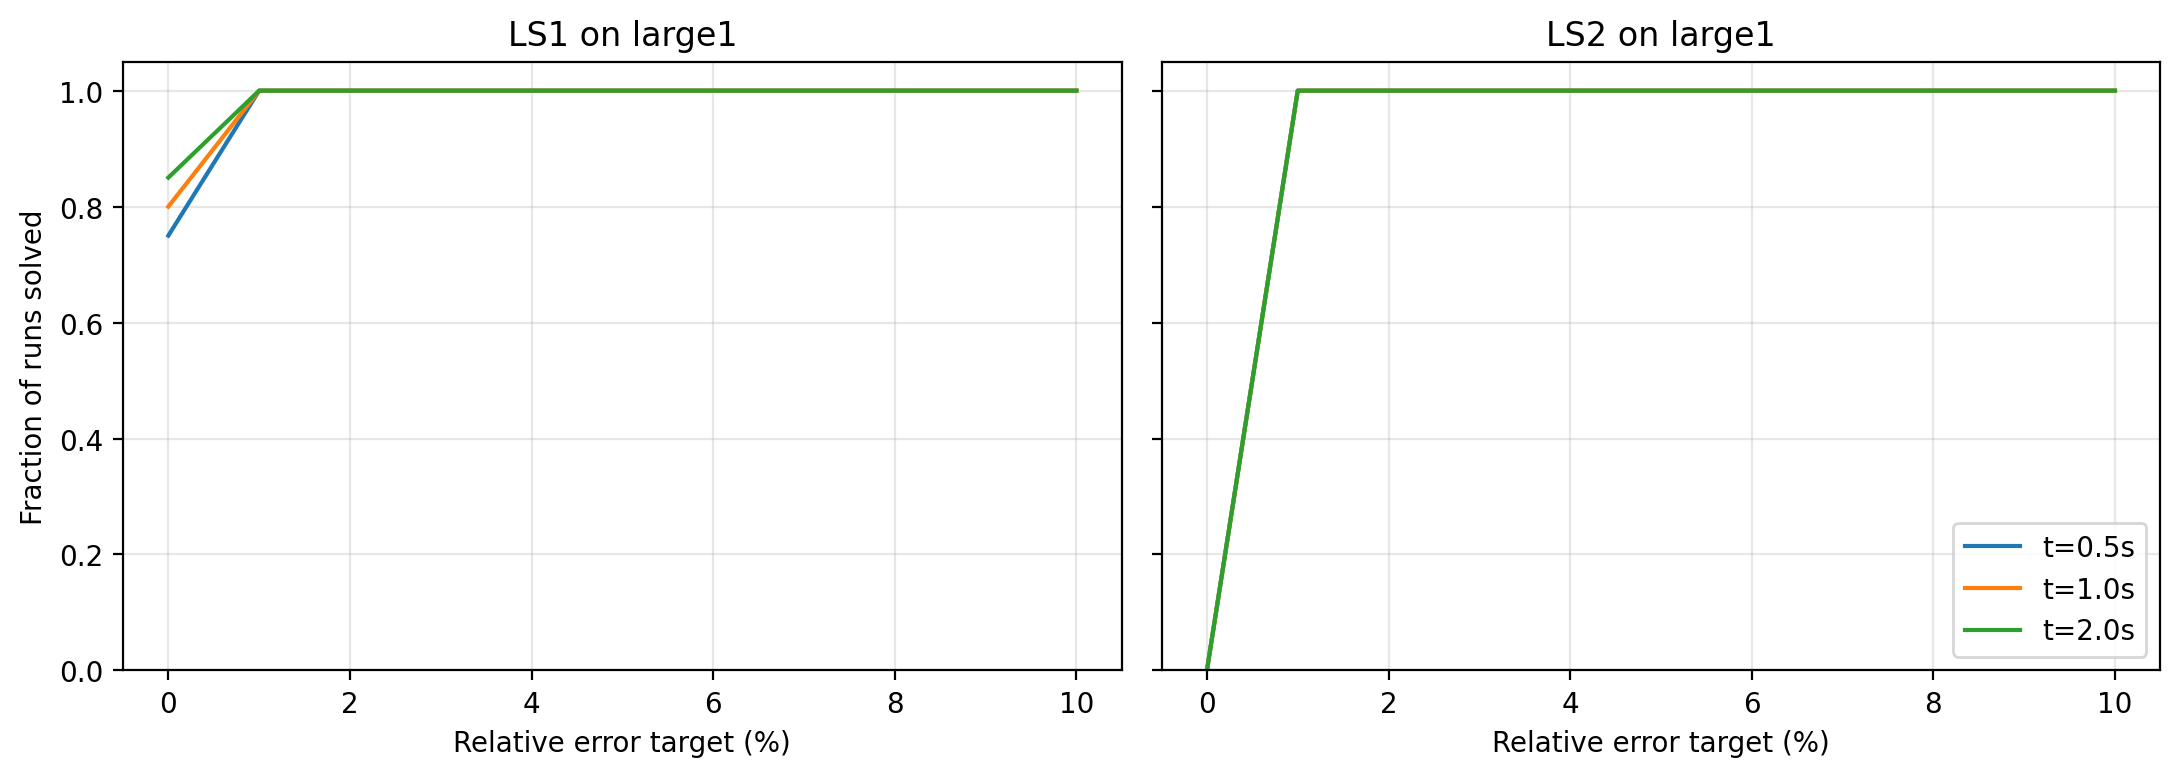
\includegraphics[width=\textwidth]{figures/sqd_large1.png}
\caption{SQD curves for \texttt{large1}.}
\Description{Solution quality distribution curves for LS1 and LS2 on large1, showing the fraction of runs that reach varying relative-error targets by each time point.}
\end{figure}

\begin{figure}[H]
\centering
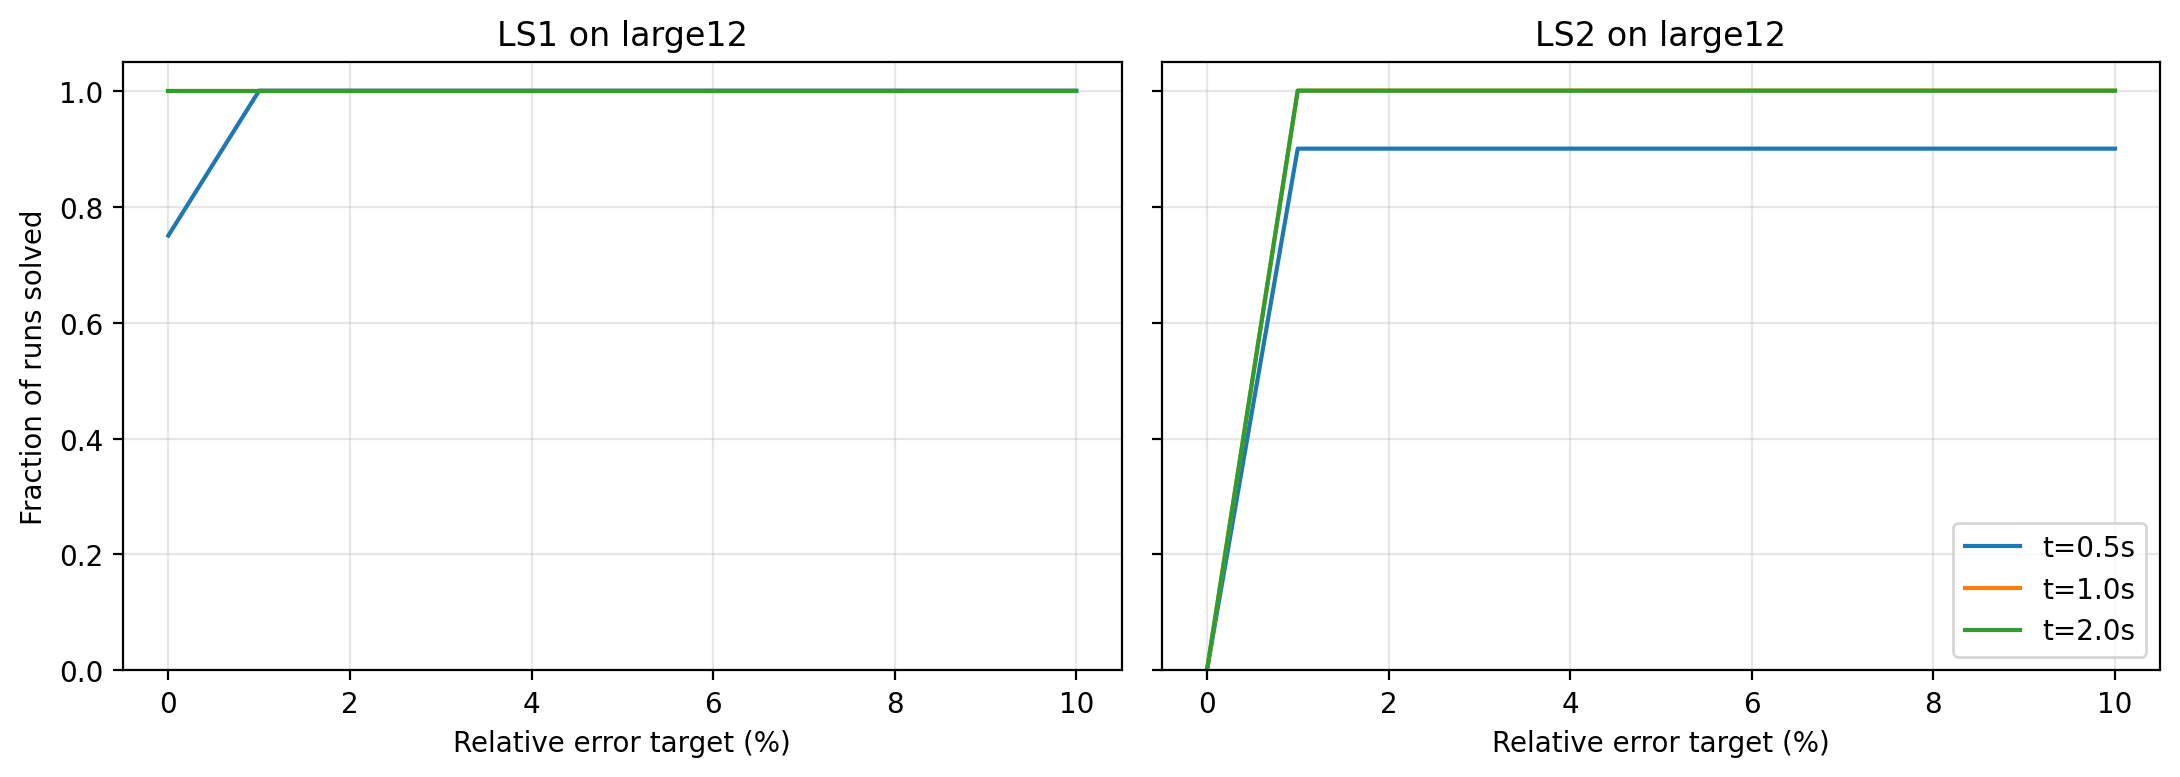
\includegraphics[width=\textwidth]{figures/sqd_large12.png}
\caption{SQD curves for \texttt{large12}.}
\Description{Solution quality distribution curves for LS1 and LS2 on large12, showing the fraction of runs that reach varying relative-error targets by each time point.}
\end{figure}

\begin{figure}[H]
\centering
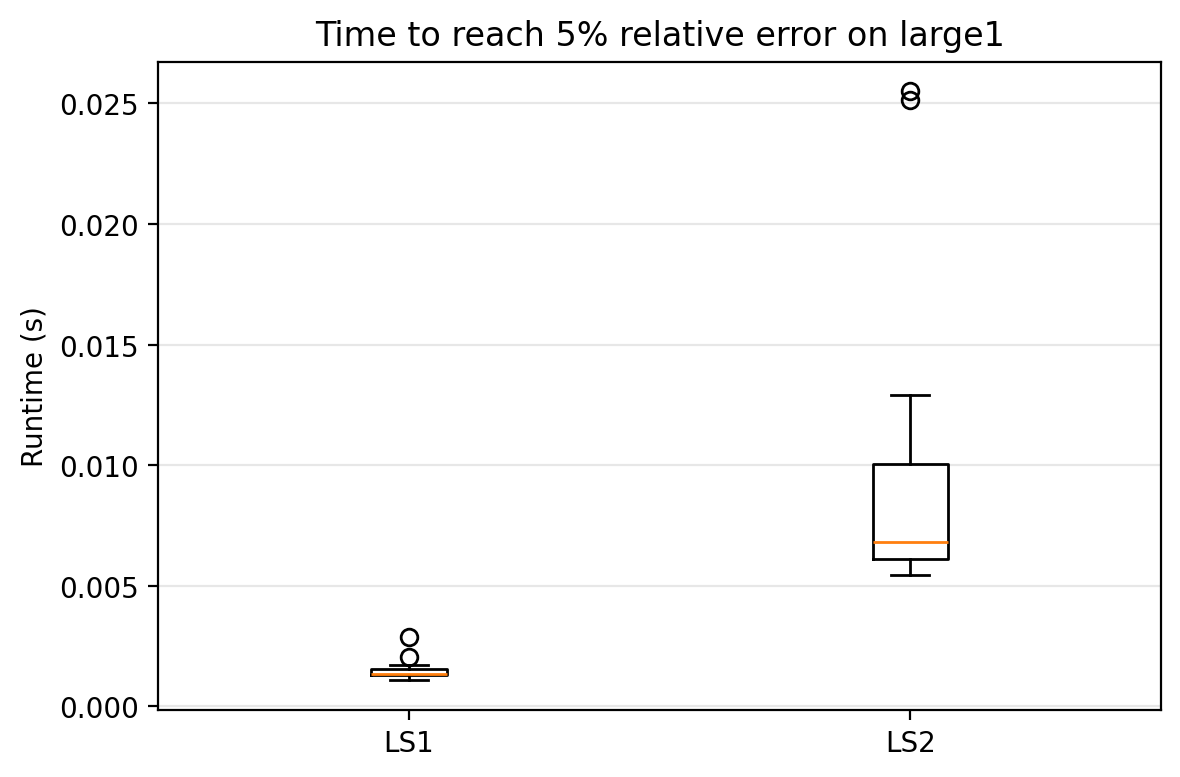
\includegraphics[width=0.75\textwidth]{figures/boxplot_large1.png}
\caption{Box plot of time to reach 5\% relative error on \texttt{large1}.}
\Description{A box plot comparing LS1 and LS2 on large1 using the runtime required to reach 5 percent relative error, with unsuccessful runs clipped at the two-second cutoff.}
\end{figure}

\begin{figure}[H]
\centering
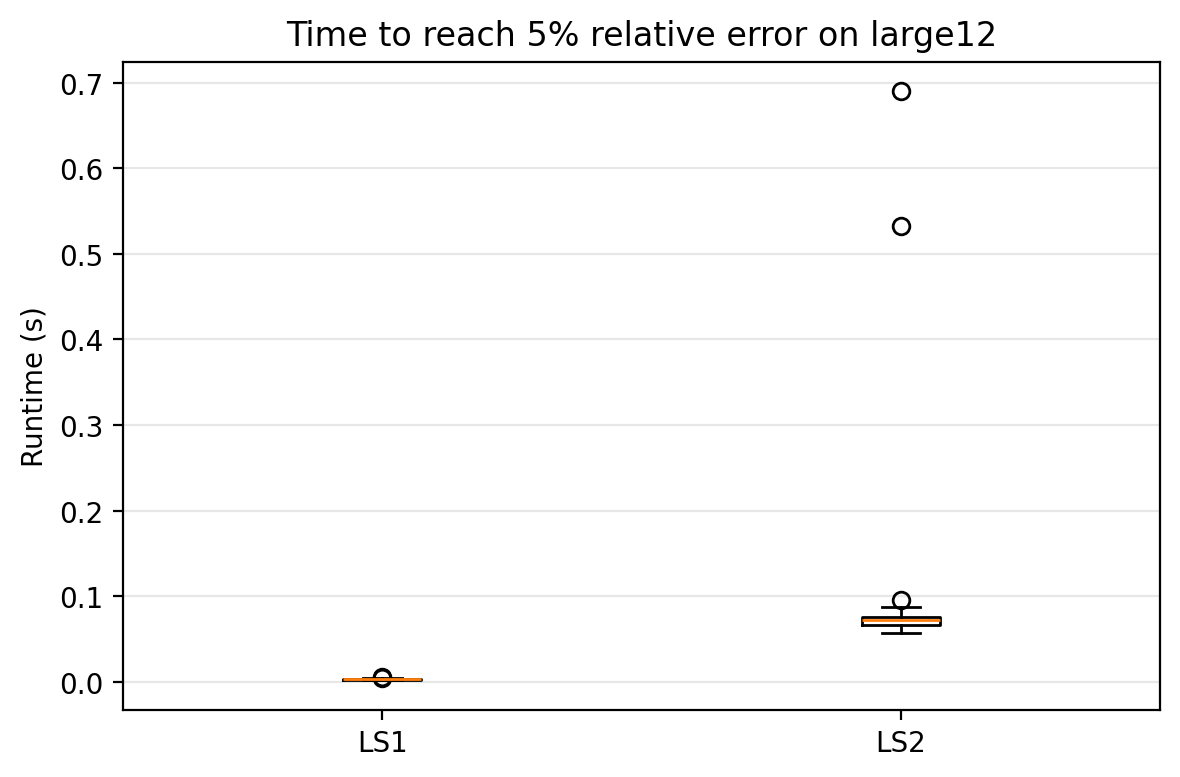
\includegraphics[width=0.75\textwidth]{figures/boxplot_large12.png}
\caption{Box plot of time to reach 5\% relative error on \texttt{large12}.}
\Description{A box plot comparing LS1 and LS2 on large12 using the runtime required to reach 5 percent relative error, with unsuccessful runs clipped at the two-second cutoff.}
\end{figure}

\end{document}
